% =============================================================================
% CHƯƠNG 3 — CÔNG NGHỆ QUẢN LÝ DỮ LIỆU, XỬ LÝ DỮ LIỆU VÀ QUY TRÌNH KIỂM CHỨNG
% Nội dung đối chiếu với repo marketpulse-360 @ dbe614b.
% =============================================================================

Chương này trình bày bốn cụm công nghệ cốt lõi của MarketPulse 360. Mỗi cụm được mô tả theo cùng một trình tự: công nghệ là gì và đóng vai trò gì, nó vận hành ra sao trong hệ thống, và những điểm hiện thực đáng chú ý. Cuối chương là năm ví dụ minh họa truy vết trực tiếp trên dữ liệu và mã nguồn.

\section{Apache Kafka và Apicurio Registry}
\label{sec:c3-kafka}

\subsection{Định nghĩa và vai trò}
\label{sec:c3-kafka-dinh-nghia}
Apache Kafka là nền tảng truyền dữ liệu phân tán dựa trên \emph{nhật ký chỉ ghi thêm} (append-only log)~\cite{kreps2011kafka, kafkadocs}. Mỗi topic được chia thành nhiều partition; bản ghi trong một partition có thứ tự và được định vị bằng offset, nên người tiêu thụ có thể đọc lại từ bất kỳ vị trí nào. Trong MarketPulse 360, Kafka 4.3.1 chạy ở chế độ KRaft (không cần ZooKeeper) và đóng vai trò \emph{trục sự kiện chung}: mọi sự kiện đều đi qua Kafka trước khi được nhánh luồng và nhánh lô tiêu thụ. Hai nhánh không độc lập hoàn toàn, vì nhánh lô dựng tầng Silver từ đầu ra của Flink (Mục~\ref{sec:c3-lakehouse-co-che}). Apicurio Registry 3.3.3~\cite{apicurio} lưu các hợp đồng dữ liệu (JSON Schema) có phiên bản cho từng topic.

\subsection{Cơ chế hoạt động}
\label{sec:c3-kafka-co-che}
Hệ thống dùng mười topic có phiên bản \texttt{v1}, chia thành bốn nhóm theo mức độ xử lý (Bảng~\ref{tab:kafka-topics}). Topic \texttt{raw} nhận dữ liệu nguồn từ công cụ phát lại; topic \texttt{clean} và \texttt{gold} do Flink ghi ra; hai topic \texttt{dlq} chứa bản ghi lỗi ở phía producer và phía Flink. Khóa phân vùng được chọn theo khóa nghiệp vụ: ưu tiên \texttt{customer\_id}, nếu không có thì dùng \texttt{session\_id}, \texttt{order\_id} hoặc \texttt{message\_id} tùy topic. Kafka chỉ giữ thứ tự trong một partition, nên cách chọn khóa này bảo đảm thứ tự cho các sự kiện cùng khóa trong cùng một topic: mọi sự kiện của một khách đã định danh nằm chung một partition, còn sự kiện của khách ẩn danh được nhóm theo phiên. Vì vậy, các phiên khác nhau của cùng một thiết bị ẩn danh có thể nằm ở các partition khác nhau, và Kafka không bảo đảm thứ tự giữa các topic.

\begin{table}[H]
\centering
\caption{Cấu hình các Kafka topic}
\label{tab:kafka-topics}
\footnotesize
\renewcommand{\arraystretch}{1.2}
\begin{tabularx}{\textwidth}{>{\raggedright\arraybackslash}p{6.3cm} >{\centering\arraybackslash}p{1.6cm} >{\raggedright\arraybackslash}p{2.6cm} >{\raggedright\arraybackslash}X}
\toprule
\textbf{Topic} & \textbf{Partition} & \textbf{Chính sách lưu} & \textbf{Khóa / bên ghi} \\
\midrule
\texttt{marketing.raw.web-events.v1} & 6 & delete, 7 ngày & khách hàng hoặc phiên; replay \\
\texttt{marketing.raw.order-events.v1} & 6 & delete, 7 ngày & khách hàng hoặc đơn hàng; replay \\
\texttt{marketing.raw.email-events.v1} & 6 & delete, 7 ngày & khách hàng hoặc email; replay \\
\texttt{marketing.dlq.validation.v1} & 6 & delete, 7 ngày & ca lỗi; replay \\
\texttt{marketing.clean.customer-events.v1} & 6 & delete, 7 ngày & \texttt{identity\_key}; Flink \\
\texttt{marketing.clean.sessions.v1} & 6 & compact, delete, 7 ngày & phiên; Flink \\
\texttt{marketing.gold.funnel-metrics.v1} & 3 & compact, delete, 30 ngày & \texttt{metric\_key}; Flink \\
\texttt{marketing.gold.revenue-metrics.v1} & 3 & compact, delete, 30 ngày & \texttt{metric\_key}; Flink \\
\texttt{marketing.gold.campaign-metrics.v1} & 3 & compact, delete, 30 ngày & \texttt{metric\_key}; Flink \\
\texttt{marketing.dlq.flink-validation.v1} & 6 & delete, 7 ngày & mã lỗi; Flink \\
\bottomrule
\end{tabularx}
\end{table}

Topic phiên và topic \texttt{gold} dùng chính sách \emph{compact}: Kafka chỉ giữ giá trị mới nhất của mỗi khóa, phù hợp với dữ liệu dạng ``trạng thái hiện tại'' như chỉ số của một chiến dịch trong ngày. Trước khi phát lại, mười hợp đồng JSON Schema được đăng ký lên Apicurio: hợp đồng chưa có thì tạo mới, hợp đồng đã có chỉ được thêm phiên bản khi nội dung thật sự thay đổi.

\subsection{Điểm nổi bật trong MarketPulse 360}
\label{sec:c3-kafka-hien-thuc}
\begin{itemize}
    \item \textbf{Gửi lại không tạo bản sao.} Producer bật \texttt{enable.idempotence} và \texttt{acks=all}; nếu một lần gửi bị lỗi và producer tự gửi lại trong cùng phiên, Kafka không ghi thêm bản sao vào partition. Bảo đảm này chỉ áp dụng cho việc gửi lại; bản ghi trùng có sẵn trong dữ liệu nguồn vẫn đi vào Kafka và được Flink, Silver khử trùng sau đó.
    \item \textbf{Phát lại an toàn.} Con trỏ phát lại lưu vị trí đã gửi và gắn với mã băm của manifest dữ liệu. Nếu xác nhận gửi không rõ ràng hoặc thế giới dữ liệu đã thay đổi, công cụ dừng lại thay vì đoán.
    \item \textbf{Tách biệt hợp đồng và dữ liệu.} Hợp đồng JSON Schema được quản lý tập trung, giúp bản ghi lỗi bị chặn ngay ở cửa vào và được chuyển sang DLQ thay vì làm hỏng các bảng phía sau.
\end{itemize}

\section{Apache Flink}
\label{sec:c3-flink}

\subsection{Định nghĩa và vai trò}
\label{sec:c3-flink-dinh-nghia}
Apache Flink là động cơ xử lý luồng phân tán có trạng thái~\cite{carbone2015flink, flinkdocs}. Flink xử lý từng sự kiện ngay khi đến, cho phép lưu trạng thái theo khóa và khôi phục trạng thái đó sau sự cố nhờ cơ chế checkpoint nhất quán~\cite{carbone2017state}. Flink hỗ trợ \emph{thời gian sự kiện} với watermark (ý tưởng xuất phát từ mô hình Dataflow~\cite{akidau2015dataflow}) nên xử lý đúng cả khi sự kiện đến không theo thứ tự. Trong MarketPulse 360, Flink 2.2.1 là bộ não của nhánh luồng: làm sạch sự kiện và tính chỉ số chiến dịch trong vài giây.

\subsection{Cơ chế hoạt động}
\label{sec:c3-flink-co-che}
Job \texttt{marketpulse-stream-v1} gồm một chuỗi toán tử có định danh ổn định (Hình~\ref{fig:flink}):

\begin{enumerate}
    \item \textbf{Đọc và gán thời gian sự kiện.} Nguồn Kafka đọc ba topic \texttt{raw}; watermark cho phép sự kiện lệch tối đa 5 phút và đánh dấu partition nhàn rỗi sau 1 phút để watermark không bị kẹt.
    \item \textbf{Kiểm tra hợp đồng.} Bản ghi không đúng hợp đồng được tách sang side output và ghi vào \texttt{marketing.dlq.flink-validation.v1} kèm mã lỗi, không làm dừng job.
    \item \textbf{Khử trùng lặp.} Luồng được phân theo \texttt{event\_id}; trạng thái \texttt{ValueState} ghi nhớ sự kiện đã thấy trong 7 ngày (TTL \num{604800000} ms) và loại mọi bản sao.
    \item \textbf{Phân loại sự kiện trễ.} Sự kiện đến sau watermark nhưng trong ngưỡng sửa 10 phút vẫn được cập nhật vào chỉ số; sự kiện trễ hơn được ghi nhận để kiểm toán.
    \item \textbf{Gom phiên.} Theo \texttt{session\_id}, bộ hẹn giờ theo thời gian sự kiện đóng phiên sau 30 phút không hoạt động.
    \item \textbf{Chỉ số chiến dịch.} Theo \texttt{metric\_key} (chiến dịch $\times$ ngày), trạng thái tích lũy số phiên ở từng bước phễu, số đơn, doanh thu gộp, hoàn tiền và doanh thu ròng.
    \item \textbf{Ghi exactly-once.} Một sink Kafka duy nhất định tuyến bản ghi tới đúng topic và ghi theo giao thức two-phase commit với tiền tố giao dịch \texttt{marketpulse-flink-v1-}. Checkpoint chạy mỗi 5 giây ở chế độ exactly-once.
\end{enumerate}

\begin{figure}[!htbp]
    \centering
    \resizebox{\textwidth}{!}{\input{chapters/Figs/fig-flink-topology}}
    \caption{Topology chuỗi toán tử xử lý luồng có trạng thái trên Apache Flink}
    \label{fig:flink}
\end{figure}

\subsection{Điểm nổi bật trong MarketPulse 360}
\label{sec:c3-flink-hien-thuc}
Điểm quan trọng nhất là \emph{tính nhất quán khi có sự cố}. Offset nguồn, trạng thái khử trùng, trạng thái phiên và chỉ số chiến dịch được lưu trong cùng một checkpoint, còn kết quả chỉ hiển thị cho người đọc sau khi giao dịch Kafka được commit. Vì vậy, khi một TaskManager bị khởi động lại, job tiếp tục từ checkpoint gần nhất mà không đếm thiếu hay đếm trùng (Ví dụ~1, Mục~\ref{sec:c3-vi-du-1}). Mọi toán tử đều có \texttt{uid} cố định, nên có thể nâng cấp job mà vẫn khôi phục được trạng thái cũ. Bộ gửi job cũng được thiết kế lũy đẳng: nó nhận ra job đang chạy ở mọi trạng thái chưa kết thúc và không tạo job thứ hai.

\section{Lakehouse: MinIO, Iceberg, Nessie và Spark}
\label{sec:c3-lakehouse}

\subsection{Định nghĩa và vai trò}
\label{sec:c3-lakehouse-dinh-nghia}
Kiến trúc \emph{lakehouse} kết hợp chi phí thấp của hồ dữ liệu với tính giao dịch của kho dữ liệu~\cite{armbrust2021lakehouse}. MarketPulse 360 hiện thực kiến trúc này bằng bốn thành phần: MinIO là kho đối tượng tương thích S3~\cite{minio}; Apache Iceberg 1.12.0 là định dạng bảng mở với snapshot có giao dịch và phân vùng ẩn~\cite{icebergspec}; Project Nessie 0.109.0 là catalog quản lý danh mục bảng~\cite{nessie}; Apache Spark 4.0.4 là động cơ tính toán lô~\cite{zaharia2012rdd, sparkdocs}.

\subsection{Cơ chế hoạt động}
\label{sec:c3-lakehouse-co-che}
\textbf{Tầng Bronze.} Bronze lưu năm topic: ba topic \texttt{raw}, topic \texttt{clean.customer-events} và topic \texttt{dlq.flink-validation} của Flink; các topic \texttt{gold} không được lưu vì có thể tính lại từ Silver. Spark đọc Kafka ở chế độ \texttt{read\_committed} theo một khoảng offset xác định, nên chỉ thấy bản ghi của giao dịch đã commit. Mỗi lần chạy đọc tiếp từ offset lớn nhất đã có trong Bronze đến offset mới nhất trên broker. Retention 7 ngày của Kafka vì vậy cũng là ràng buộc của nhánh lô: nếu nhánh lô ngừng chạy lâu hơn 7 ngày, các offset cần đọc có thể đã bị Kafka xóa, và lần chạy dừng với lỗi \texttt{Kafka retention gap} (cấu hình \texttt{failOnDataLoss=true}) thay vì âm thầm bỏ sót dữ liệu; khi đó phải phát lại dữ liệu từ nguồn. Bản ghi đã vào Bronze thì được lưu lâu dài trên Iceberg. Việc ghi dùng \texttt{MERGE} theo khóa \texttt{ingest\_id}; nếu cùng một khóa xuất hiện với nội dung khác, quá trình dừng với lỗi va chạm khóa bất biến. File nguồn được kiểm tra kích thước và mã băm so với manifest trước khi lưu.

\textbf{Tầng Silver.} Spark giải mã các sự kiện \texttt{clean}, gom các bản sao theo \texttt{event\_id} và chọn bản thắng theo thứ tự xác định. Phiên bản 1 của hợp đồng \texttt{clean} không mang \texttt{click\_id}, nên Silver nối ngược về bản ghi \texttt{raw} qua bộ ba lineage để khôi phục trường này, đồng thời kiểm tra \texttt{event\_id} hai phía phải trùng nhau. Sự kiện không có đồng thuận phân tích bị loại với mã \texttt{CONSENT\_DENIED}, sự kiện bị Flink đánh dấu trễ quá ngưỡng bị loại với mã \texttt{LATE\_INELIGIBLE}, phiên bot web/app bị loại với mã \texttt{BOT\_EXCLUDED}; mọi quyết định đều được đếm trong \texttt{silver.quality\_summary}.

\textbf{Phụ thuộc giữa nhánh lô và Flink.} Vì Silver dựng \texttt{silver.customer\_events} từ topic \texttt{clean}, nhánh lô kế thừa các quyết định của Flink: kết quả kiểm tra hợp đồng, cách phân loại sự kiện trễ và giá trị các trường đã chuẩn hóa. Silver có một lớp đối soát với dữ liệu gốc: mọi offset của topic \texttt{raw} phải có đúng một kết cục (nằm trong \texttt{clean}, nằm trong DLQ, hoặc là bản sao của một sự kiện đã nhận), thiếu một offset là cả lô thất bại. Tuy nhiên, Silver không tự tính lại giá trị của từng trường từ dữ liệu \texttt{raw}. Nếu Flink có lỗi logic, chẳng hạn chuẩn hóa sai số tiền, lỗi đó sẽ đi vào số liệu đã kiểm chứng. Trên dữ liệu mô phỏng, lớp kiểm tra độc lập với Flink là oracle story-demo: nó tính lại các chỉ số trực tiếp từ file nguồn của bộ sinh, không đi qua đường ống, và phát hiện được loại lỗi này (Mục~\ref{sec:c5-oracle}). Với dữ liệu thật, cần bổ sung một phép đối soát giá trị độc lập giữa \texttt{raw} và \texttt{clean} (Mục~\ref{sec:c6-huong-phat-trien}).

\textbf{Tầng Gold.} Spark xây dựng sáu bảng phân tích. Phép phân bổ doanh thu tìm các click trả phí của cùng hồ sơ trong cửa sổ 30 ngày trước đơn hàng, rồi chia tiền theo ba mô hình First-Touch, Last-Touch và Linear; đơn hàng không có điểm chạm nào được gán cho \texttt{\_\_unattributed\_\_} để tổng tiền luôn bảo toàn.

\subsection{Điểm nổi bật trong MarketPulse 360}
\label{sec:c3-lakehouse-hien-thuc}
\begin{itemize}
    \item \textbf{Tái lập theo snapshot.} Mỗi lần chuẩn bị dữ liệu sinh một \emph{phiếu chuẩn bị} (preparation receipt) ghi lại mã snapshot của từng bảng Bronze, Silver và Gold. Nhờ truy vấn theo phiên bản của Iceberg (\texttt{VERSION AS OF}), mọi tính toán sau đó đều đọc đúng trạng thái đã ghim, kể cả khi bảng nguồn đã có dữ liệu mới.
    \item \textbf{Không gian tên cô lập.} Mỗi lần chuẩn bị ghi Silver và Gold vào một namespace riêng \texttt{mp\_batch\_<identity>\_<attempt>}, nên một lần chạy lỗi không bao giờ làm hỏng kết quả trước đó.
    \item \textbf{Tiền là số nguyên.} Mọi số tiền được lưu bằng đơn vị nhỏ nhất (VND) kiểu \texttt{long}; phép chia luôn là phép chia nguyên có phân bổ phần dư (Ví dụ~3).
    \item \textbf{Phân vùng phù hợp truy vấn.} Bảng sự kiện phân vùng theo tháng, bảng Kafka phân vùng theo ngày, giúp truy vấn lịch sử và tính lại chỉ quét đúng phần dữ liệu liên quan.
\end{itemize}

\section{Dagster, dbt và ClickHouse}
\label{sec:c3-dagster-dbt-clickhouse}

\subsection{Định nghĩa và vai trò}
\label{sec:c3-dagster-dinh-nghia}
Dagster 1.13 là công cụ điều phối theo mô hình \emph{tài sản dữ liệu định nghĩa bằng phần mềm} (Software-Defined Assets): thay vì mô tả các tác vụ, người phát triển mô tả các bảng cần có và phụ thuộc giữa chúng~\cite{dagsterdocs}. dbt Core 1.12 biến đổi dữ liệu bằng SQL có quản lý phiên bản và chạy kiểm thử dữ liệu như kiểm thử phần mềm~\cite{dbtdocs}. ClickHouse 26.8 là CSDL lưu theo cột tối ưu cho truy vấn phân tích, dùng họ động cơ bảng MergeTree~\cite{clickhousedocs}.

\subsection{Cơ chế hoạt động}
\label{sec:c3-dagster-co-che}
Đồ thị gồm 13 định nghĩa tài sản chia thành ba giai đoạn (Hình~\ref{fig:dagster}). Lịch \texttt{daily\_marketing\_refresh} chạy lúc 02:00 hằng ngày cho ngày hôm trước thông qua job \texttt{marketing\_refresh\_job}. Job \texttt{historical\_rebuild\_job} chạy lại toàn bộ đồ thị trừ bước công bố, dùng để tính lại lịch sử một cách cô lập; job \texttt{source\_history\_job} nạp lần đầu dữ liệu nguồn cho các ngày quá khứ.

\begin{figure}[H]
    \centering
    \resizebox{\textwidth}{!}{\input{chapters/Figs/fig-dagster}}
    \caption{Đồ thị phụ thuộc các tài sản dữ liệu trên Dagster}
    \label{fig:dagster}
\end{figure}

Sau khi Gold được xây xong, snapshot được xuất thành file JSON kèm manifest có checksum, rồi nạp vào một CSDL ClickHouse \emph{ứng viên} mới tinh \texttt{mp\_release\_<identity>\_<attempt>}. Tám bảng \texttt{raw\_*} trong CSDL này là nguồn của dbt; dbt dựng chín mô hình và chạy 31 bài kiểm thử (Bảng~\ref{tab:dbt}). Chỉ khi mọi bước của quy trình trong Hình~\ref{fig:certification} thành công, bản phát hành mới được công bố.

\begin{figure}[H]
    \centering
    \resizebox{\textwidth}{!}{% Hình 3.3 — Kiểm chứng bản phát hành cô lập và công bố nguyên tử
\begin{tikzpicture}[node distance=5mm, s/.style={mpbox=37mm, minimum height=19mm}]
  % Hàng 1: chuẩn bị và dựng ứng viên
  \node[s] (p1) {\textbf{1. Phiếu chuẩn bị}\\ ghim snapshot Bronze\\ \texttt{identity} = SHA-256};
  \node[s, right=of p1] (p2) {\textbf{2. Xuất snapshot}\\ file JSON + manifest\\ có checksum, lưu MinIO};
  \node[s, right=of p2] (p3) {\textbf{3. Nạp ứng viên}\\ CSDL \texttt{mp\_release\_*}\\ 8 bảng \texttt{raw\_*}};
  \node[s, right=of p3] (p4) {\textbf{4. dbt build}\\ 9 mô hình\\ 31 bài kiểm thử};
  % Hàng 2: đối soát và công bố (đi ngược từ phải sang trái)
  \node[s, below=8mm of p4] (p5) {\textbf{5. Đối soát checksum}\\ checksum từng bảng\\ oracle CTR/CPC\\ \texttt{proof\_digest}};
  \node[s, left=of p5] (p6) {\textbf{6. Ghi sổ cái}\\ \texttt{certified\_bundles}\\ \texttt{publications}\\ (PostgreSQL)};
  \node[s, left=of p6] (p7) {\textbf{7. Công bố}\\ \texttt{publication\_journal}\\ (ClickHouse)};
  \node[mphead=37mm, minimum height=19mm, left=of p7] (p8) {Ứng dụng đọc\\ \texttt{max(generation)}};
  % Nhánh thất bại
  \node[mpbox=60mm, below=8mm of p6, xshift=-21mm, draw=mpline, fill=mpzone] (fail)
    {\textbf{Bất kỳ bước nào thất bại}\\ ứng viên bị loại bỏ, release đang phục vụ giữ nguyên};

  \draw[mparrow] (p1) -- (p2);
  \draw[mparrow] (p2) -- (p3);
  \draw[mparrow] (p3) -- (p4);
  \draw[mparrow] (p4) -- (p5);
  \draw[mparrow] (p5) -- (p6);
  \draw[mparrow] (p6) -- (p7);
  \draw[mparrow] (p7) -- (p8);
  \draw[mpdash] (p5.south) |- (fail.east);
\end{tikzpicture}
}
    \caption{Quy trình kiểm chứng bản phát hành cô lập và công bố nguyên tử}
    \label{fig:certification}
\end{figure}

\subsection{Tầng Gold và các mô hình dbt}
\label{sec:c3-gold-schema}
Hình~\ref{fig:schema-gold} và Hình~\ref{fig:schema-gold-2} trình bày chín mô hình trong CSDL release, với kiểu dữ liệu ClickHouse. Sáu mô hình là bản sao chính xác của các bảng Iceberg \texttt{gold.*}; \texttt{campaigns} và \texttt{customers} là hai bảng chiều xuất từ Silver; \texttt{campaign\_dashboard} là mart làm giàu từ \texttt{campaign\_performance\_daily} (32 cột) và \texttt{campaigns}, bổ sung tên, trạng thái chiến dịch, CTR và CPC. Khóa ngoại tới \texttt{campaigns} được kiểm thử bởi \texttt{campaign\_relationships}, ngoại trừ giá trị đặc biệt \texttt{\_\_unattributed\_\_}; khóa ngoại tới \texttt{customers} được kiểm thử bởi \texttt{customer\_relationships}. Bảng \texttt{cohort\_retention} được tổng hợp từ \texttt{customer\_360} và hoạt động theo tháng nên được biểu diễn bằng quan hệ dẫn xuất.

\begin{figure}[!htbp]
    \centering
    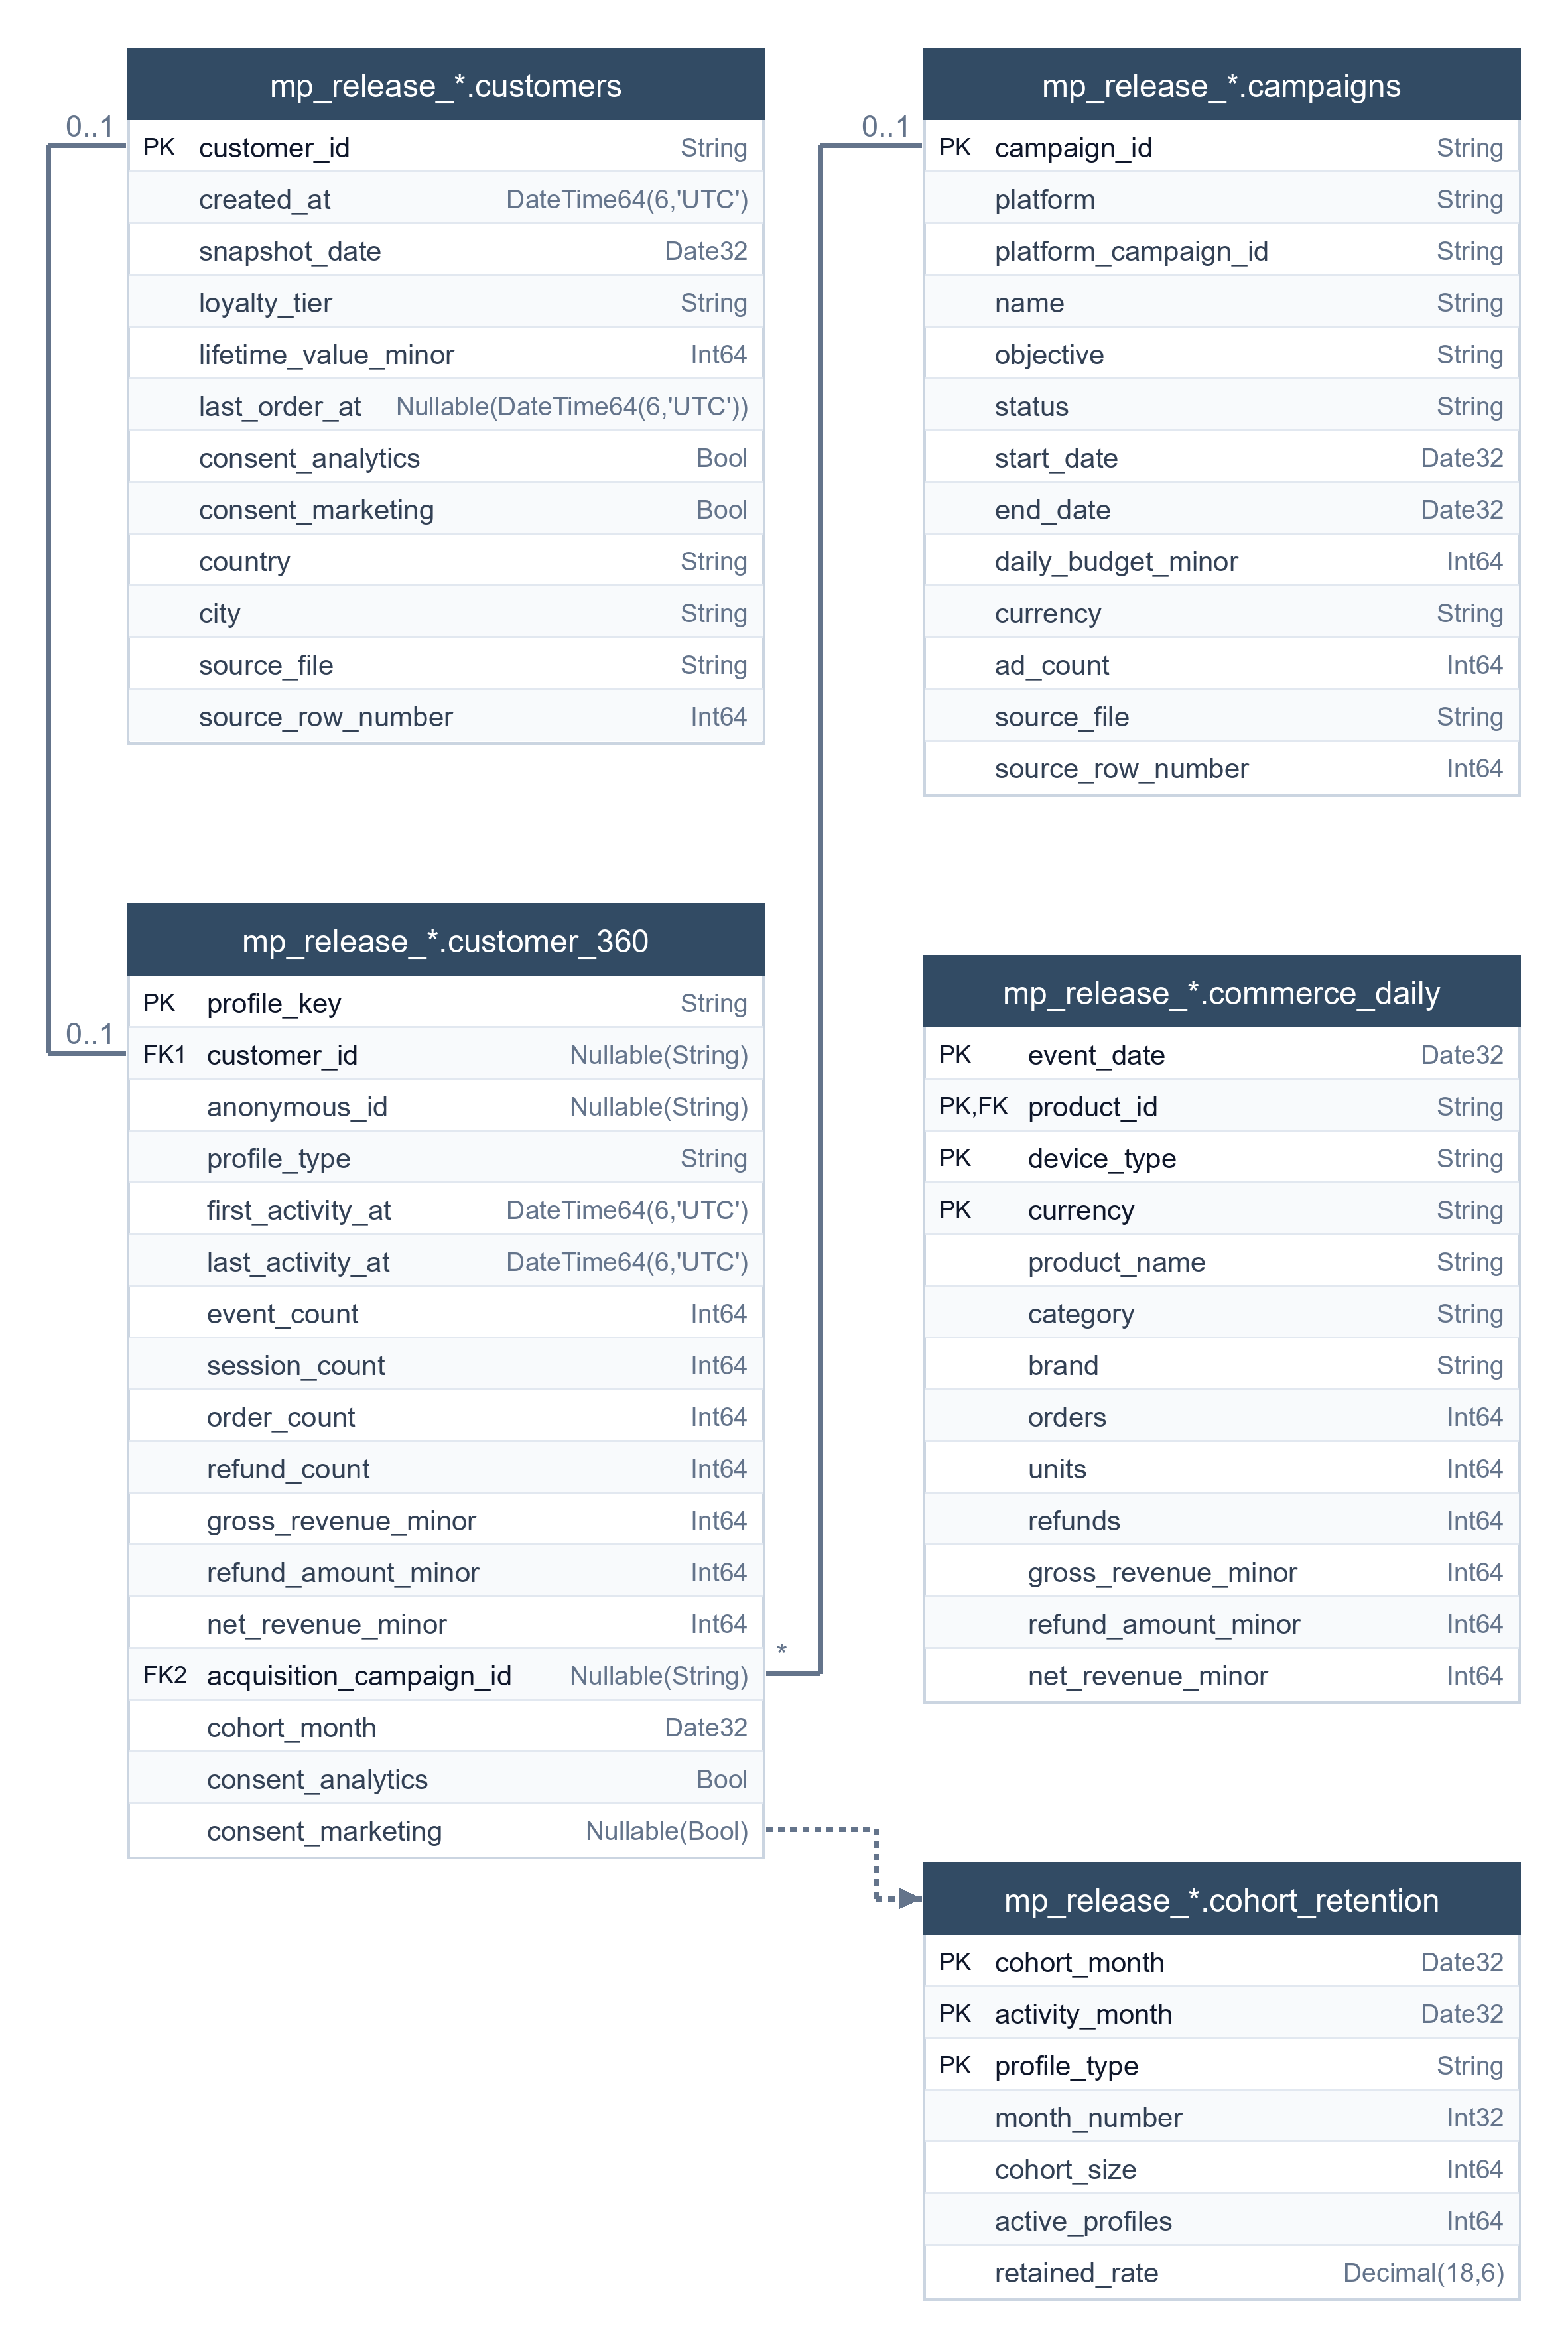
\includegraphics[width=\textwidth, height=0.86\textheight, keepaspectratio]{chapters/Pics/schema-gold-1.png}
    \caption{Lược đồ quan hệ các mô hình dbt phục vụ trên ClickHouse (phần 1): bảng chiều, Customer 360, thương mại và cohort}
    \label{fig:schema-gold}
\end{figure}

\begin{figure}[!htbp]
    \centering
    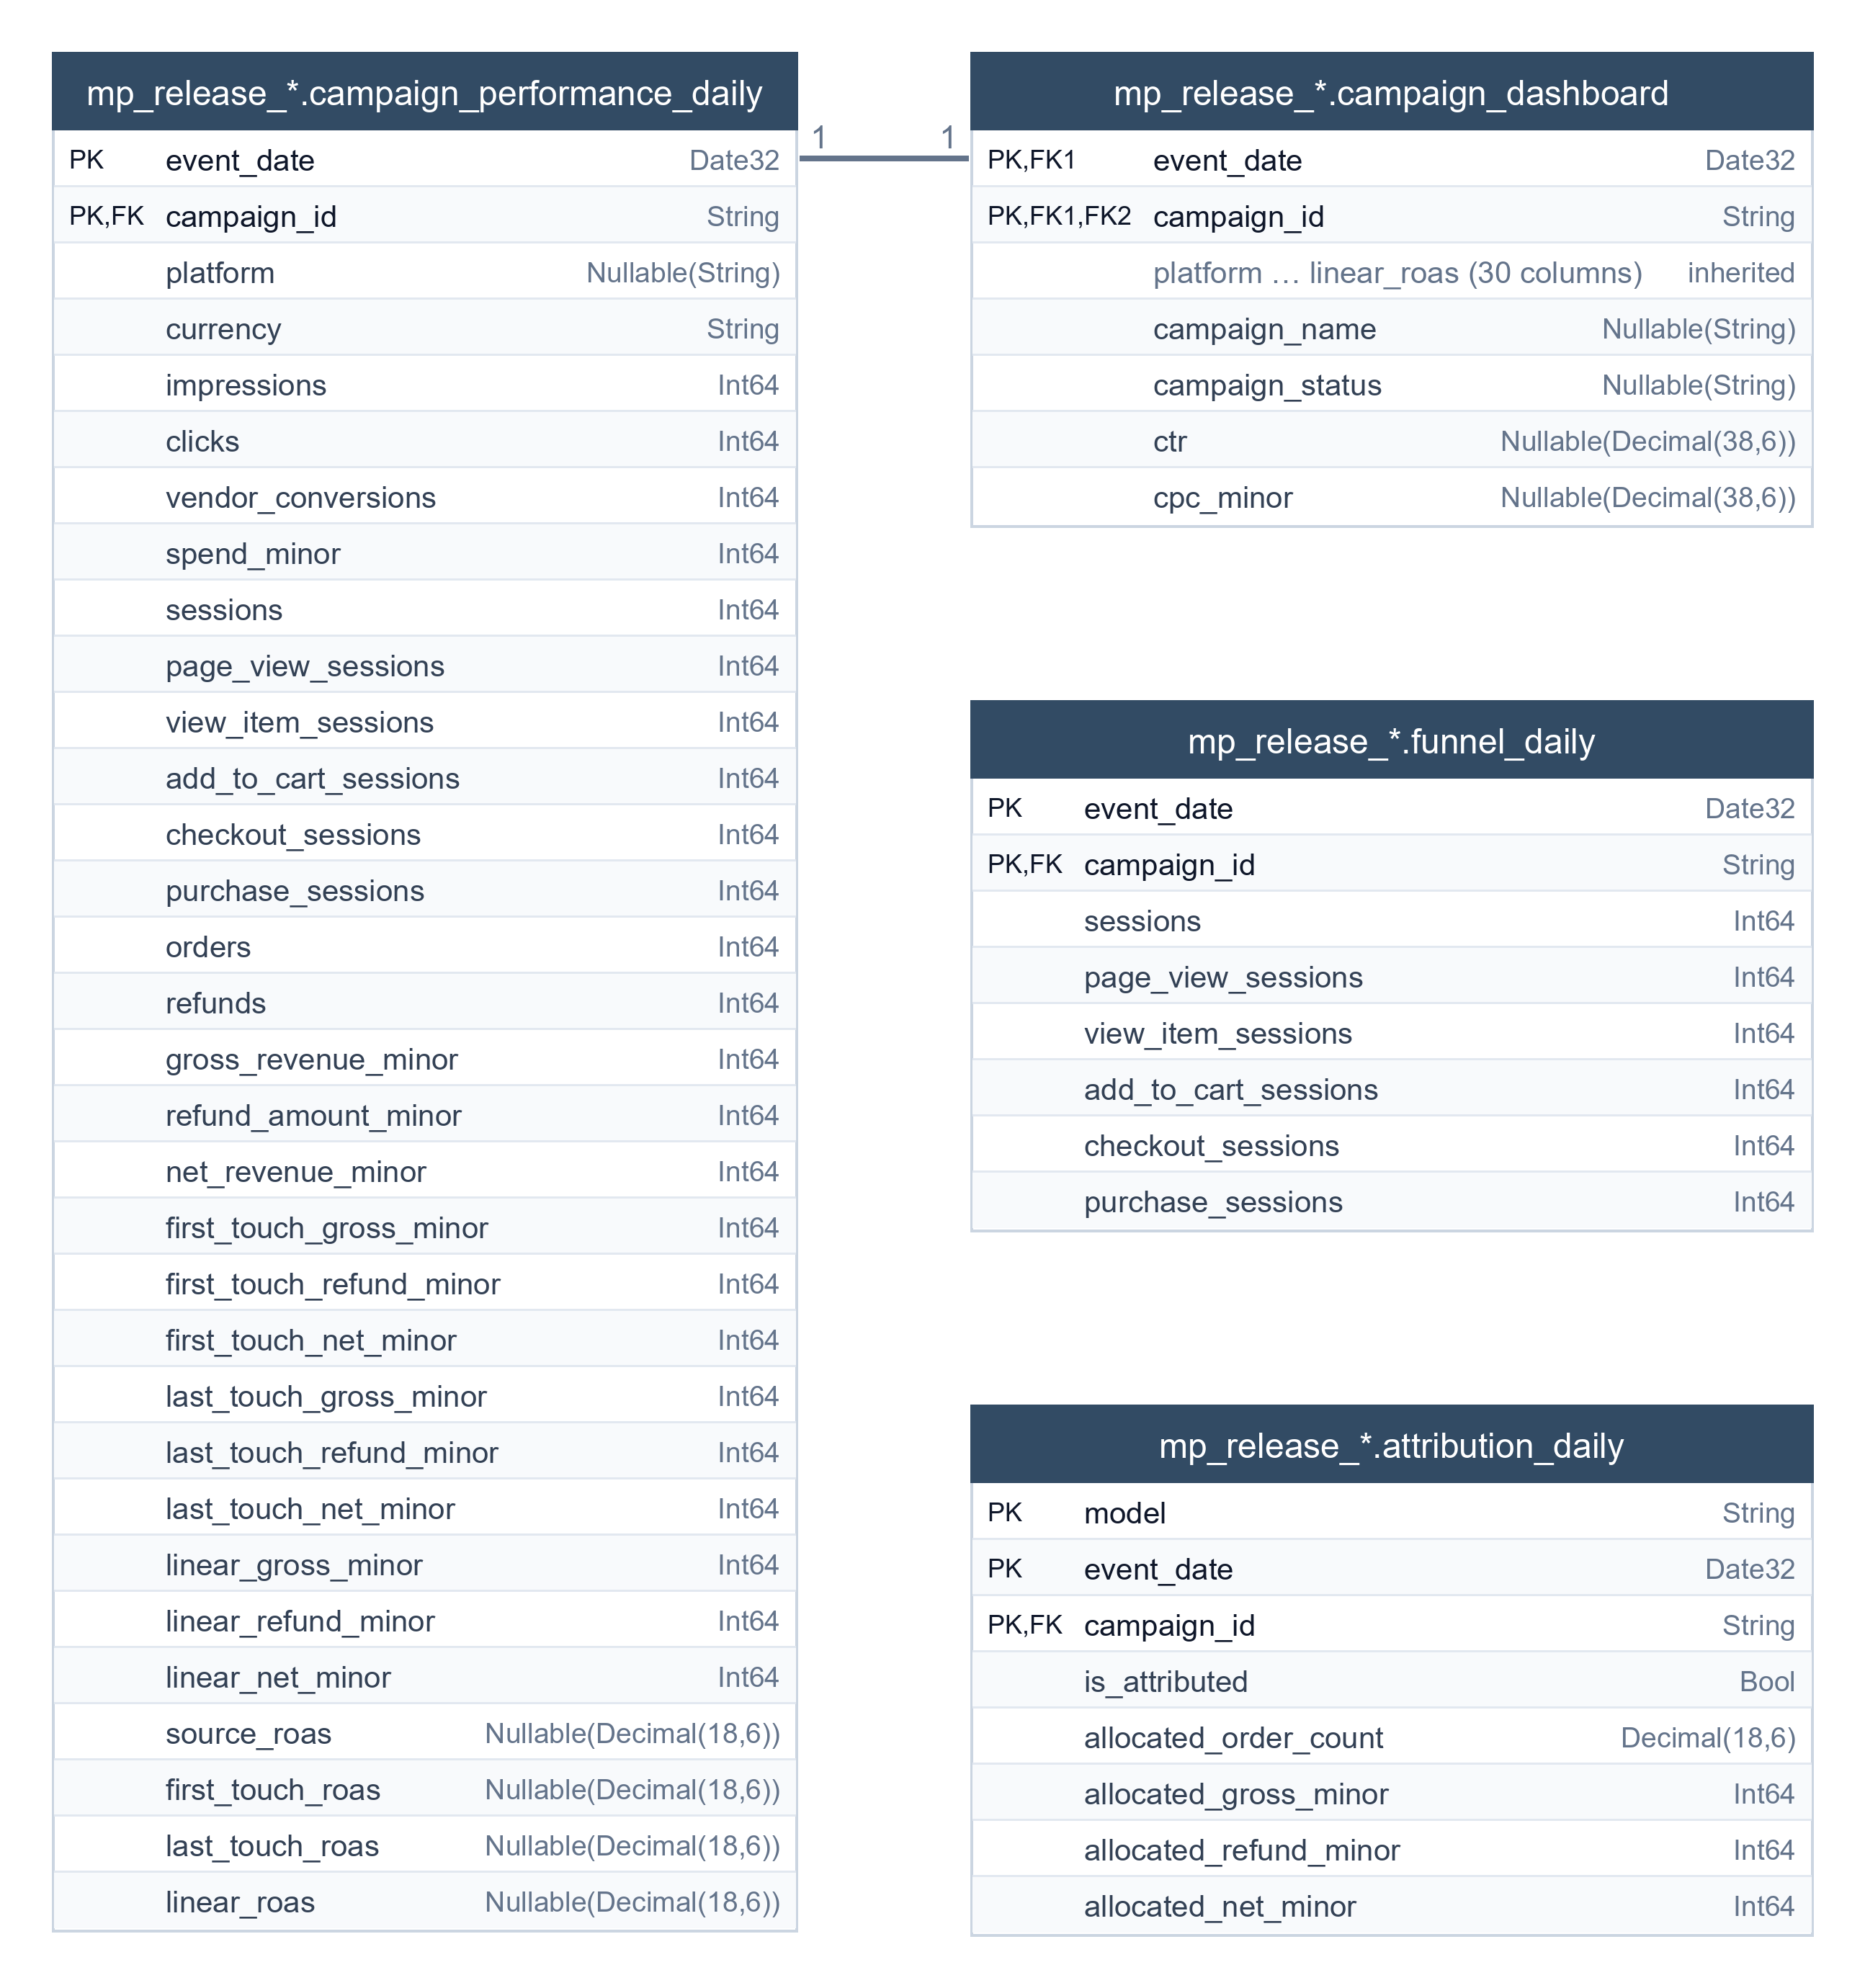
\includegraphics[width=\textwidth, height=0.86\textheight, keepaspectratio]{chapters/Pics/schema-gold-2.png}
    \caption[Lược đồ quan hệ các mô hình dbt phục vụ trên ClickHouse (phần 2): hiệu quả chiến dịch, phễu và phân bổ]{Lược đồ quan hệ các mô hình dbt phục vụ trên ClickHouse (phần 2): hiệu quả chiến dịch, phễu và phân bổ. Cột \texttt{campaign\_id} của bốn bảng là khóa ngoại tới \texttt{campaigns} ở Hình~\ref{fig:schema-gold}}
    \label{fig:schema-gold-2}
\end{figure}

\begin{table}[!htbp]
\centering
\caption{Các mô hình dbt và bài kiểm thử chất lượng dữ liệu tự động}
\label{tab:dbt}
\footnotesize
\renewcommand{\arraystretch}{1.2}
\begin{tabularx}{\textwidth}{>{\raggedright\arraybackslash}p{5.0cm} >{\raggedright\arraybackslash}p{5.7cm} >{\raggedright\arraybackslash}X}
\toprule
\textbf{Mô hình (ORDER BY)} & \textbf{Nguồn} & \textbf{Kiểm thử tổng quát} \\
\midrule
\texttt{campaign\_performance\_daily} & \texttt{raw\_campaign\_performance\_daily} & khóa duy nhất, cột bắt buộc \\
\texttt{funnel\_daily} & \texttt{raw\_funnel\_daily} & khóa duy nhất, cột bắt buộc, not null \\
\texttt{attribution\_daily} & \texttt{raw\_attribution\_daily} & khóa duy nhất, cột bắt buộc, giá trị hợp lệ \\
\texttt{customer\_360} & \texttt{raw\_customer\_360} & khóa duy nhất, cột bắt buộc, giá trị hợp lệ \\
\texttt{cohort\_retention} & \texttt{raw\_cohort\_retention} & khóa duy nhất, cột bắt buộc \\
\texttt{commerce\_daily} & \texttt{raw\_commerce\_daily} & khóa duy nhất, cột bắt buộc \\
\texttt{campaigns} & \texttt{raw\_campaigns} & khóa duy nhất, cột bắt buộc, not null \\
\texttt{customers} & \texttt{raw\_customers} & khóa duy nhất, cột bắt buộc, not null \\
\texttt{campaign\_dashboard} & \texttt{campaign\_performance\_daily} $\bowtie$ \texttt{campaigns} & khóa duy nhất \\
\midrule
\multicolumn{3}{>{\raggedright\arraybackslash}p{15.2cm}}{\textbf{Kiểm thử nghiệp vụ (9):} \texttt{financial\_equations} (gộp $-$ hoàn = ròng ở mọi bảng), \texttt{attribution\_conservation} (tổng phân bổ của mỗi mô hình bằng doanh thu Customer 360), \texttt{commerce\_conservation}, \texttt{campaign\_relationships}, \texttt{customer\_relationships}, \texttt{cohort\_invariants}, \texttt{funnel\_invariants}, \texttt{consent\_eligibility}, \texttt{accepted\_domains}.} \\
\midrule
\multicolumn{3}{l}{\textbf{Tổng cộng:} 22 kiểm thử tổng quát + 9 kiểm thử nghiệp vụ = 31 kiểm thử.} \\
\bottomrule
\end{tabularx}
\end{table}

\subsection{Điểm nổi bật trong MarketPulse 360}
\label{sec:c3-dagster-hien-thuc}
\begin{itemize}
    \item \textbf{Kiểm chứng trên dữ liệu thật của release.} Ngoài 31 bài kiểm thử dbt, bước đối soát checksum (bước 5 trong Hình~\ref{fig:certification}) tính checksum cho toàn bộ dòng của từng bảng và so với checksum lúc xuất, tính lại CTR, CPC bằng một oracle độc lập, rồi gộp mọi bằng chứng thành \texttt{proof\_digest}.
    \item \textbf{Công bố nguyên tử và đơn điệu.} Sổ cái PostgreSQL \texttt{marketpulse\_ops} giữ khóa tư vấn (advisory lock) khi đặt chỗ công bố và từ chối bản phát hành của một ngày logic cũ hơn bản đã công bố. Bản ghi được nối vào \texttt{publication\_journal} trên ClickHouse rồi mới được xác nhận; ứng dụng luôn đọc bản có \texttt{generation} lớn nhất. Một tiến trình công bố chậm vì thế không thể ``kéo lùi'' người đọc về bản cũ.
    \item \textbf{Không tái sử dụng ứng viên dở dang.} Mỗi lần nạp tạo một CSDL mới theo số lần thử; một CSDL nạp dở không bao giờ được dùng lại.
\end{itemize}

\section{Ví dụ minh họa}
\label{sec:c3-vi-du}

Năm ví dụ dưới đây được chọn để mỗi ví dụ minh họa một rủi ro điển hình của dữ liệu marketing và cách đường ống xử lý nó. Các con số đều lấy từ bằng chứng chạy thật trong kho mã~\cite{mp360repo}.

\subsection{Ví dụ 1: Khử trùng lặp và phục hồi trên Flink}
\label{sec:c3-vi-du-1}
Kịch bản kiểm thử phục hồi khởi động lại TaskManager của Flink \emph{trong khi} producer vẫn đang gửi dữ liệu, kèm hai bản sao trùng \texttt{event\_id} được chèn có chủ đích. Trong quá trình phục hồi, đầu vào Kafka thô tăng từ 83 lên 219 bản ghi. Sau khi job khôi phục từ checkpoint, đầu ra giữ đúng 217 mã sự kiện duy nhất và 73 khóa phiên, hai bản sao bị loại, và doanh thu ròng đối soát khớp \num{24751000}~VND. Kết quả cho thấy trạng thái khử trùng được khôi phục cùng offset nguồn: bản ghi đã xử lý trước sự cố không bị tính lại, bản ghi đến trong lúc sự cố không bị mất.

\subsection{Ví dụ 2: Khôi phục mã click tại tầng Silver}
\label{sec:c3-vi-du-2}
Một phiên mua hàng bắt đầu từ click quảng cáo trả phí có \texttt{click\_id} trong bản ghi \texttt{raw}, nhưng bản ghi \texttt{clean} phiên bản 1 không mang trường này. Silver dùng bộ ba \texttt{(lineage\_topic, lineage\_partition, lineage\_offset)} để tìm đúng bản ghi \texttt{raw} trong \texttt{bronze.kafka\_records}, đọc payload, kiểm tra \texttt{event\_id} trùng khớp rồi mới khôi phục \texttt{click\_id}; nhờ đó đơn hàng được phân bổ về đúng chiến dịch.

Cùng lúc, Silver áp dụng quản trị. Trên tập fixture, doanh thu ròng của luồng chưa quản trị là \num{24751000}~VND, còn doanh thu đã quản trị được công bố là \num{22193000}~VND; hai con số thuộc hai quần thể khác nhau và không được so sánh như nhau. Trên story-demo, dữ liệu nguồn có \num{33858} đơn hàng, bản phát hành đã kiểm chứng có \num{32774} đơn; chênh lệch đúng bằng \num{1084} đơn hàng có \texttt{consent\_analytics = false} và bị loại với mã \texttt{CONSENT\_DENIED}.

\subsection{Ví dụ 3: Phân bổ tuyến tính bảo toàn từng đồng}
\label{sec:c3-vi-du-3}
Giả sử một đơn hàng có doanh thu gộp $A = \num{1000000}$~VND và có $k = 3$ click trả phí trong cửa sổ 30 ngày. Mô hình Linear chia đều nhưng $\num{1000000}$ không chia hết cho 3. Hàm \texttt{allocate\_minor\_units} sắp xếp các điểm chạm theo \texttt{(event\_time, campaign\_id, click\_id, event\_id)} rồi tính
\[
  q = \left\lfloor \frac{A}{k} \right\rfloor = \num{333333}, \qquad r = A \bmod k = 1 .
\]
$r$ điểm chạm sớm nhất nhận thêm 1 đồng: phần phân bổ là \num{333334}, \num{333333}, \num{333333}~VND, tổng đúng bằng \num{1000000}~VND. Hoàn tiền được phân bổ theo cùng cách, và doanh thu ròng của mỗi phần bằng gộp trừ hoàn. Bài kiểm thử \texttt{attribution\_conservation} xác nhận tổng phân bổ của cả ba mô hình đều bằng tổng doanh thu trong \texttt{customer\_360}.

\subsection{Ví dụ 4: Chặn bản phát hành lỗi}
\label{sec:c3-vi-du-4}
Kiểm thử phương trình tài chính chỉ bắt được dòng có gộp $-$ hoàn $\neq$ ròng. Một lỗi tinh vi hơn là dữ liệu bị sửa \emph{nhất quán}: số dòng không đổi và phương trình vẫn cân. API \texttt{POST /api/v1/ops/quality/probe} (chỉ dành cho \texttt{admin}) tái hiện đúng tình huống này một cách an toàn: hệ thống sao chép release đang phục vụ sang một CSDL dùng một lần \texttt{mp09\_probe\_<uuid>}, cộng thêm 1 đồng vào cả doanh thu gộp lẫn doanh thu ròng của một dòng trong \texttt{campaign\_performance\_daily}, rồi chạy lại các phép kiểm chứng. Lỗi bị phát hiện ở hai lớp độc lập: checksum của bảng không còn khớp với checksum đã ghi lúc xuất, và tổng doanh thu không còn khớp với tổng tính trực tiếp từ sự kiện đơn hàng. Báo cáo kết luận \texttt{controlled\_same\_count\_finance\_corruption\_detected}, CSDL thử nghiệm bị xóa, còn release đang phục vụ không bị đụng tới. Trong quá trình kiểm chứng thật, các lỗi tương tự, như dòng tiền bị sửa với số dòng không đổi hoặc tham chiếu chiến dịch không tồn tại, đều làm bản ứng viên bị từ chối.

\subsection{Ví dụ 5: Tái tạo lịch sử từ Iceberg snapshot}
\label{sec:c3-vi-du-5}
Khi cần kiểm tra hoặc tính lại một ngày trong quá khứ, \texttt{historical\_rebuild\_job} đọc phiếu chuẩn bị đã lưu của ngày đó. Job chỉ chạy nếu phiên bản mô hình hiện tại trùng với phiên bản đã ghi trong phiếu; nó cấp một lần thử mới và dựng lại Silver, Gold trong namespace cô lập \texttt{mp\_batch\_<identity>\_<attempt>} từ đúng các snapshot Bronze đã ghim. Kết quả được so sánh với \texttt{proof\_digest} đã ghi; nếu khác nhau, job thất bại. Bước công bố bị bỏ qua hoàn toàn trong chế độ này, nên việc tính lại lịch sử không bao giờ thay đổi số liệu người dùng đang xem.
